\documentclass{beamer}
\usepackage{mathptmx}
\usepackage[scaled=0.9]{helvet}
\usepackage{courier}
\usetheme{CambridgeUS}
\usecolortheme{rose}
\usepackage{textpos}
\usepackage{calc}
\graphicspath{{figures/}}
\usepackage{multicol}
\usepackage{caption}
\usepackage{tikz}
\usepackage{animate}

\title[{
\includegraphics[scale=0.1]{biospytial.png}} a Graph Based Engine] % (optional, only for long titles)
{Introducing {\em Biospytial} }
\subtitle{An Open Source graph-based computing framework for managing and modelling spatial ecological data}
\author[Escamilla-Molgora et.al.] % (optional, for multiple authors)
{Juan Escamilla Molgora~\inst{1} ~\inst{2}, Luigi Sedda~\inst{3}, Peter Atkinson~\inst{1}}
\institute[Lancaster University] % (optional)
{
  \inst{1}%
	Lancaster Environment Center
  \and
  \inst{2}%
  Data Science Institute
  \and
  \inst{3}
  Faculty of Health and Medicine
}
\date[SPATSTAT2017] % (optional)
{Spatial Statistics Conference, 2017}
\subject{Computer Science}

\titlegraphic{
\includegraphics[scale=0.6]{sponsors_logo.png}}


% position the logo
\addtobeamertemplate{frametitle}{}{%
\begin{textblock*}{\paperwidth}(1cm,1cm)

\includegraphics[height=1cm,width=1cm,keepaspectratio]{biospytial.png}
\end{textblock*}}


\begin{document}
\begin{frame}
\titlepage
\end{frame}

\section{Motivations}

\begin{frame}{Ecosystems support life in Earth}
\begin{columns}[t]
        \column{.5\textwidth}
        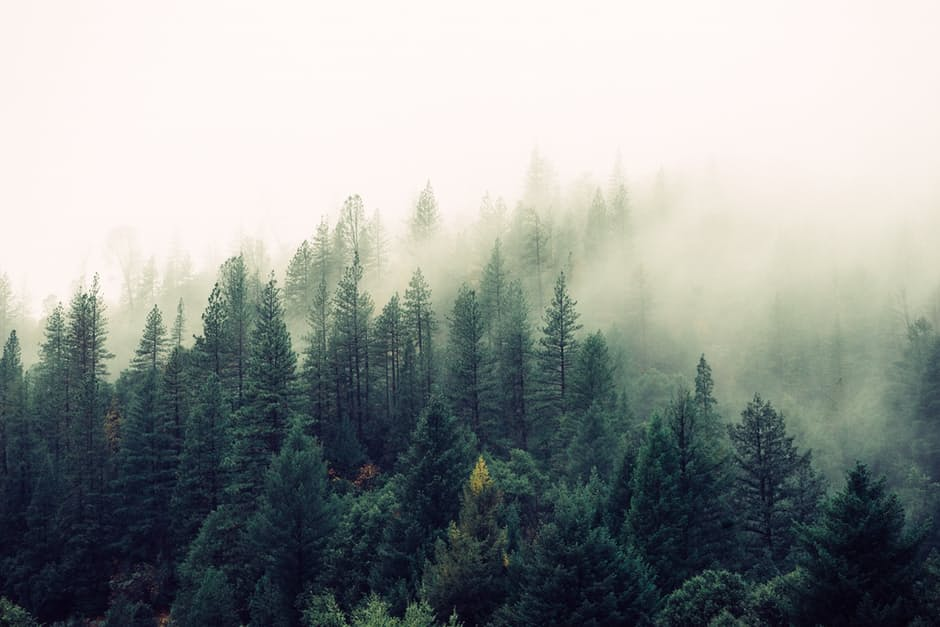
\includegraphics[width=\columnwidth,height=2.5cm]{forest1.jpeg}
        \captionof{figure}{primary production}
        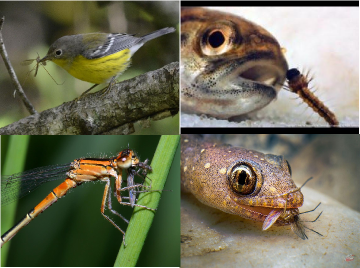
\includegraphics[width=\columnwidth,height=2.5cm]{em.png}
        \captionof{figure}{Disease regulation}
        \column{.5\textwidth}
        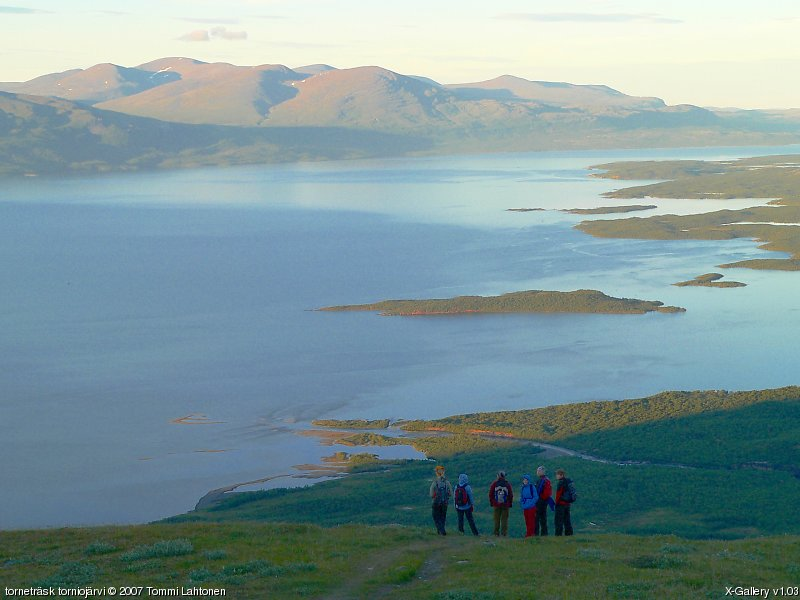
\includegraphics[width=\columnwidth,height=2.5cm]{tornetrask.jpg}
        \captionof{figure}{water cycle}
        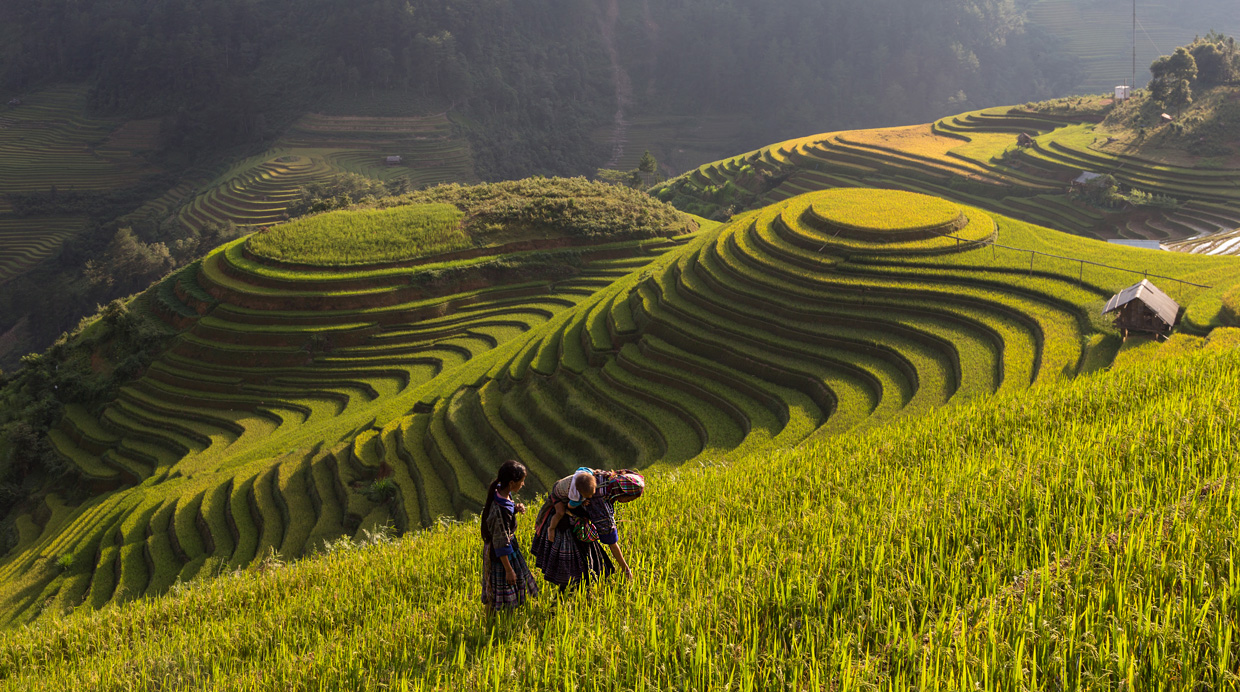
\includegraphics[width=\columnwidth,height=2.5cm]{food.jpg}
        \captionof{figure}{food supply}
\end{columns}
\end{frame}




\subsection{Why modelling?}
	\begin{frame}
		\frametitle{Why model them ?}
		\begin{block}{The environment changes}
				\begin{figure}				
				\centering
		    	\includegraphics<1>[height=0.6\textheight,width=\textwidth]{deforest1.png}	    	    
				\caption{ Landsat 5 images from June 24, 1984, and August 6, 2011. (U.S. Department of the Interior | U.S. Geological Survey)  }
		    	\end{figure}
		\end{block}
	\end{frame}

	\begin{frame}
		\frametitle{Why model them ?}
		\begin{block}{Climate Change Mitigation and Response}
				\begin{figure}				
\centering
		    	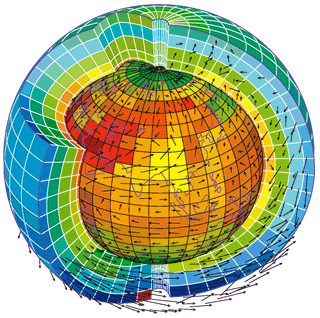
\includegraphics[width=0.4\textwidth]{ESM.png}
		    	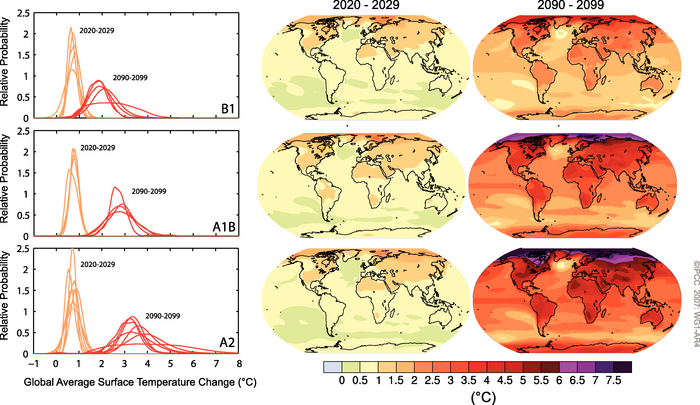
\includegraphics[width=0.6\textwidth]{ch1.png}		    	    
				\caption{Earth System Models ((L. Fairhead /LMD-CNRS) and IPCC, 2007)}
		    	\end{figure}
		\end{block}
	\end{frame}

	\begin{frame}
		\frametitle{Main question is ...}

				\begin{columns}
					\begin{column}{0.4\textwidth}
						\begin{alertblock}{Spatial regression of ecological networks}						
						\begin{itemize}
						\item<1> {\em Find the underlying process that shapes the "species"assemblages.}
						\item<2> Infer the probability of assemblages of taxa for a given location.
						\item[fig:]<3> {\small An interaction food web shows that fish have indirect effects on the populations of several species in and around ponds. }
						\end{itemize}										
					    \end{alertblock}		
					\end{column}
				
			\begin{column}{0.5\textwidth}
			\begin{figure}						
			\centering
		    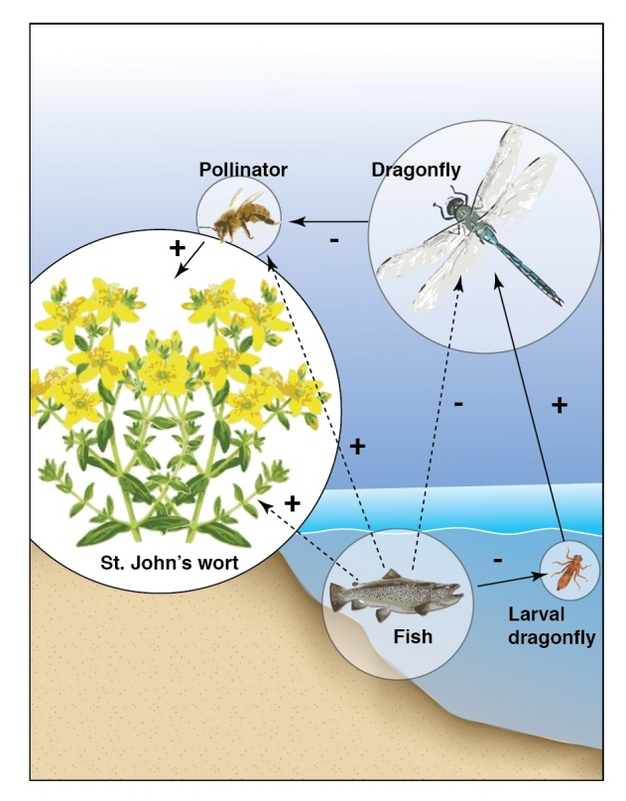
\includegraphics[scale=0.4]{foodweb2.jpg}		
		    \caption{{\small from Nature Education, 2012}}			
			\end{figure}
		    \end{column}    	    
		\end{columns}
	\end{frame}




\section{Graph based Engine}
\begin{frame}{Services and Modules}

\centering
\only<1>{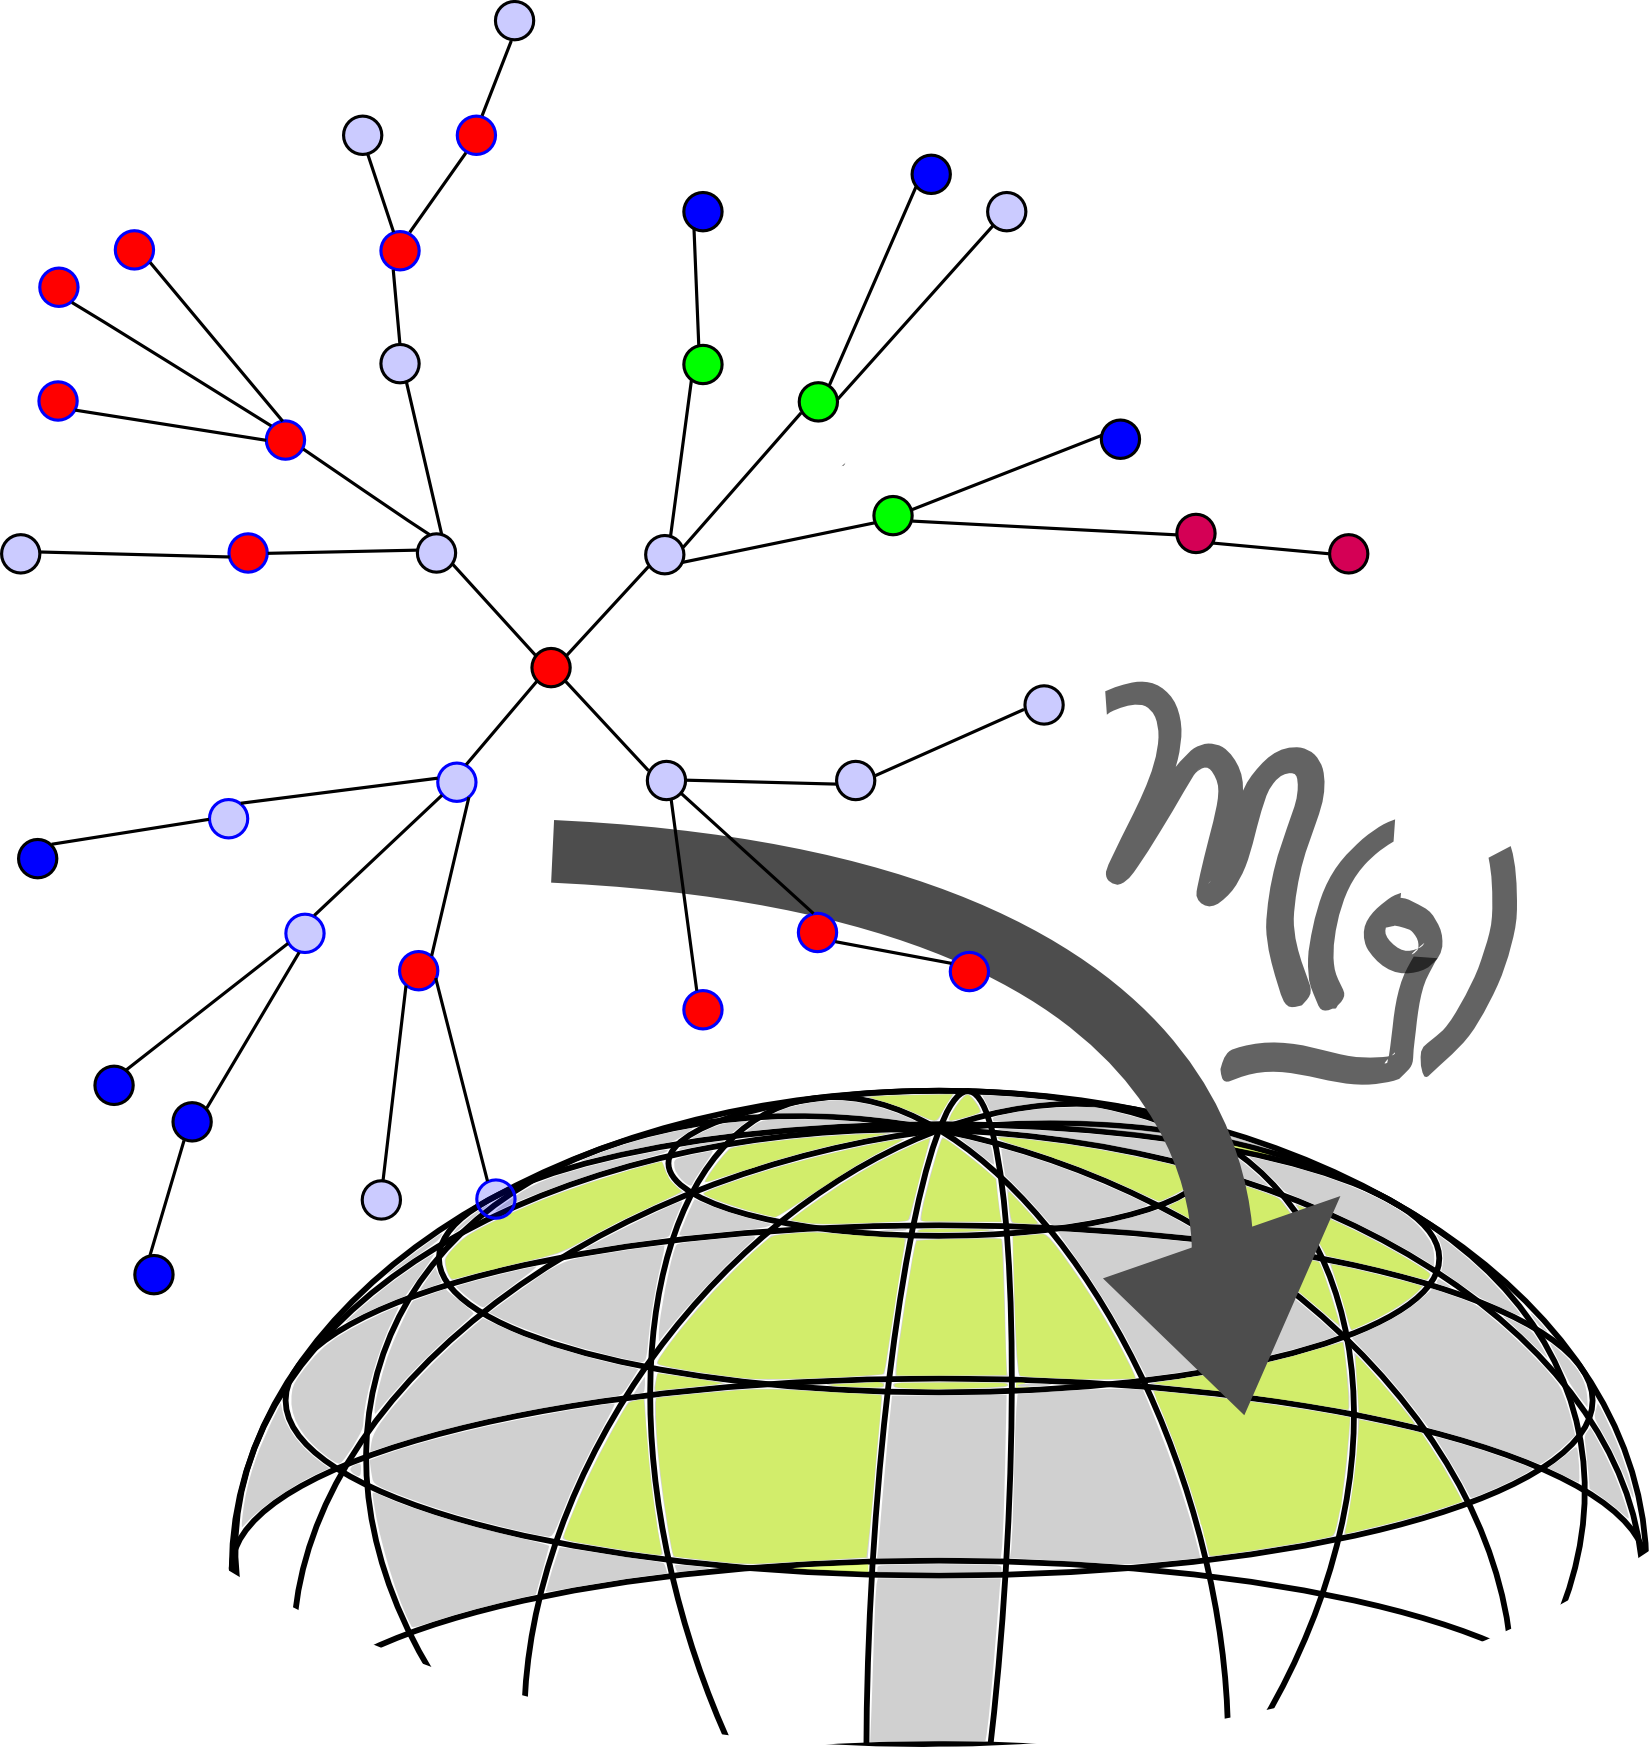
\includegraphics[scale=0.3]{graph-model.png}}
\only<2>{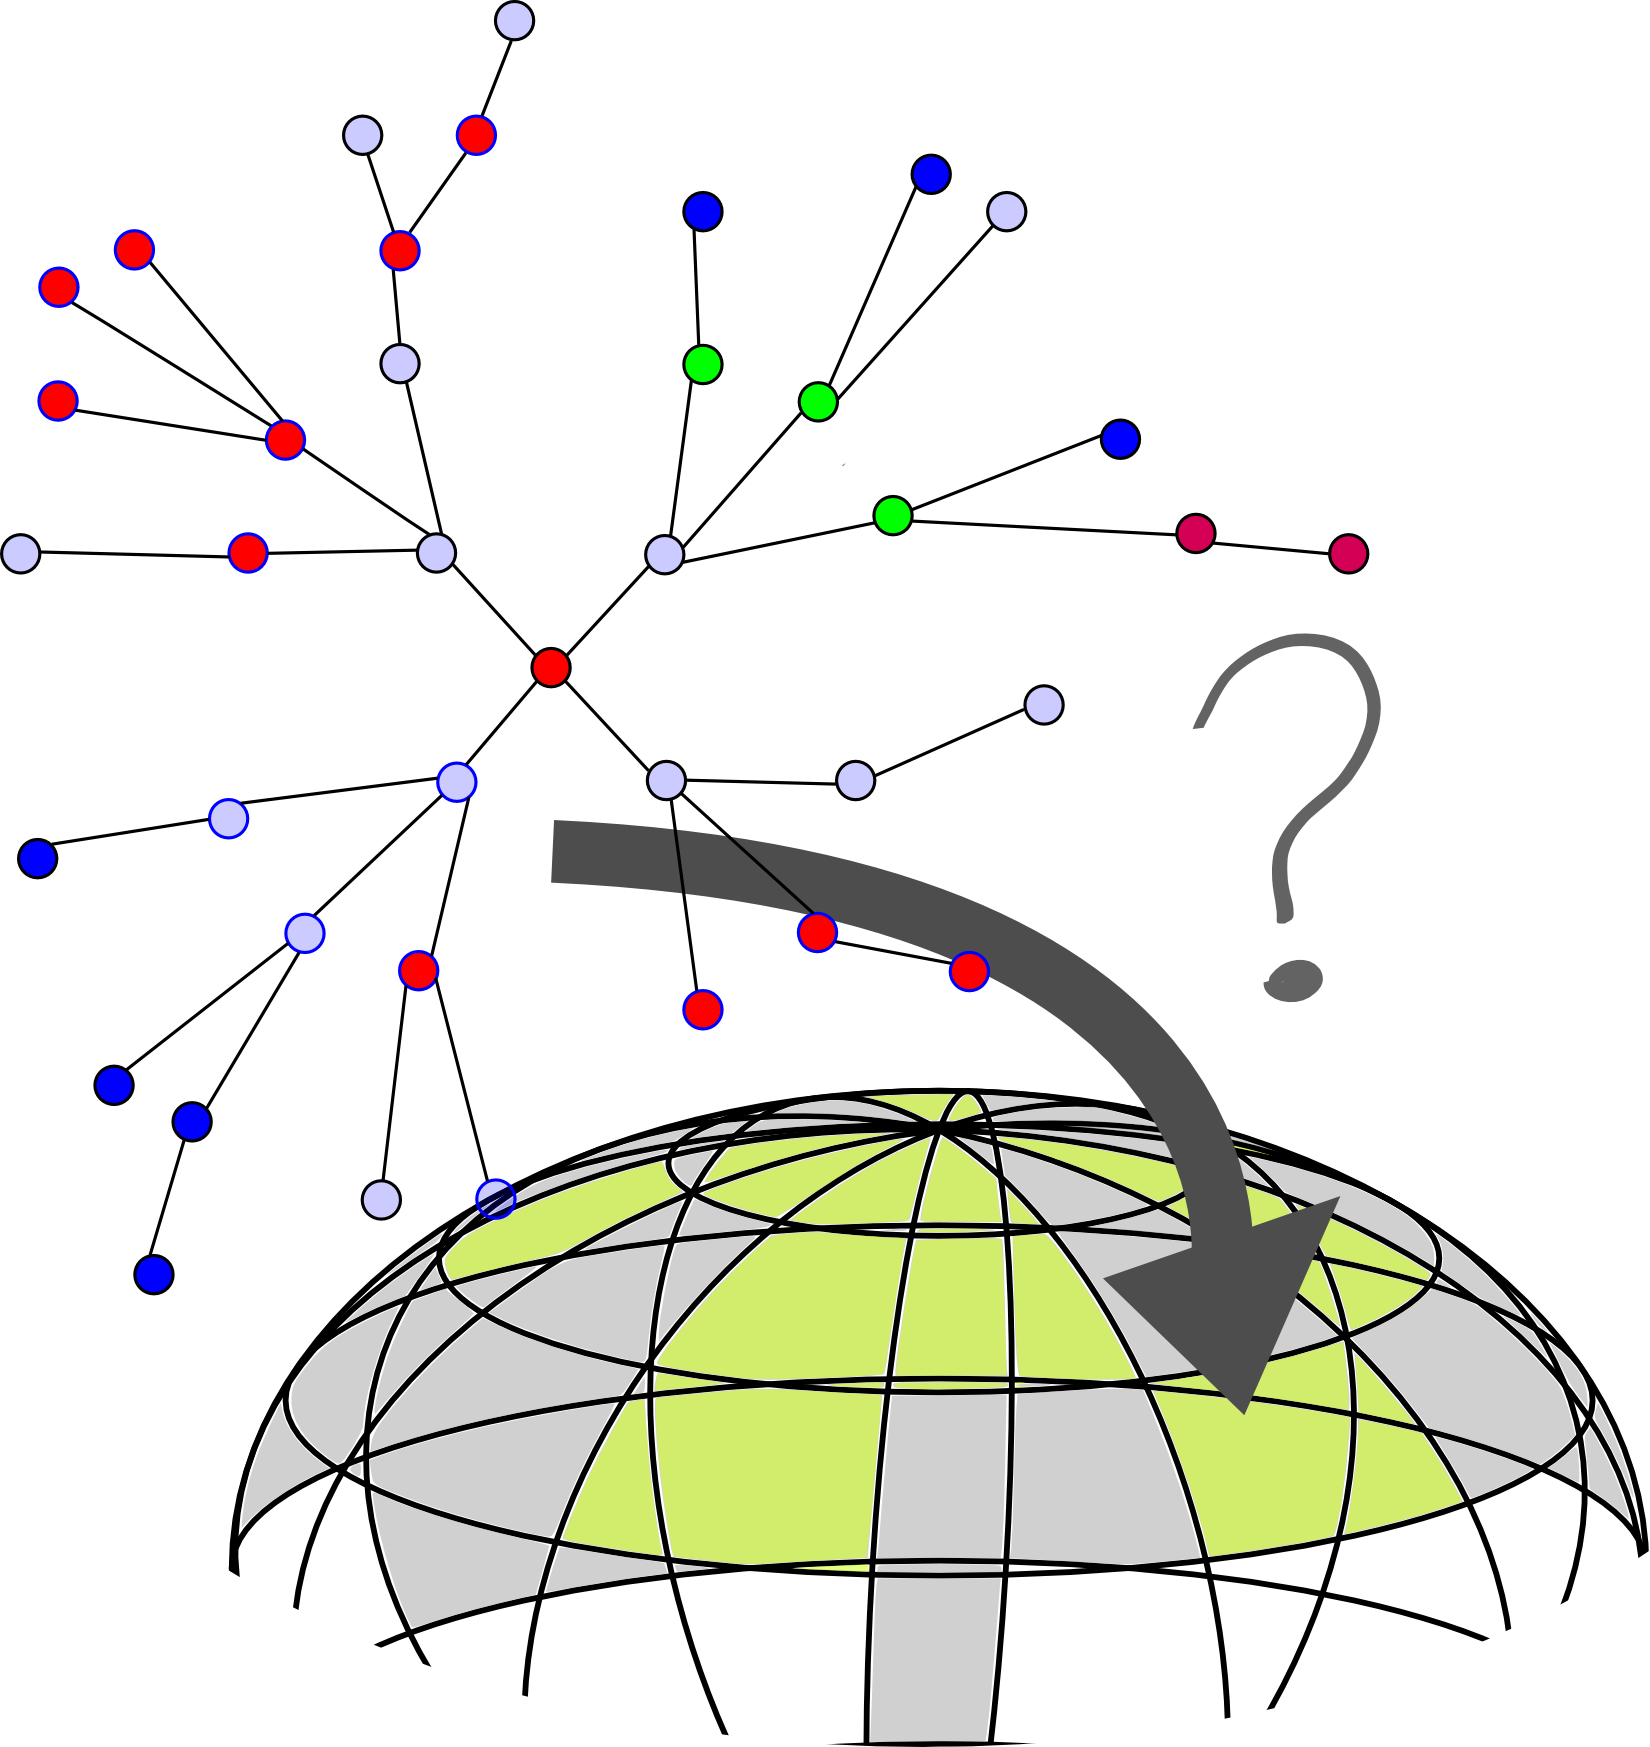
\includegraphics[scale=0.3]{graph-model2.png}}
\only<3>{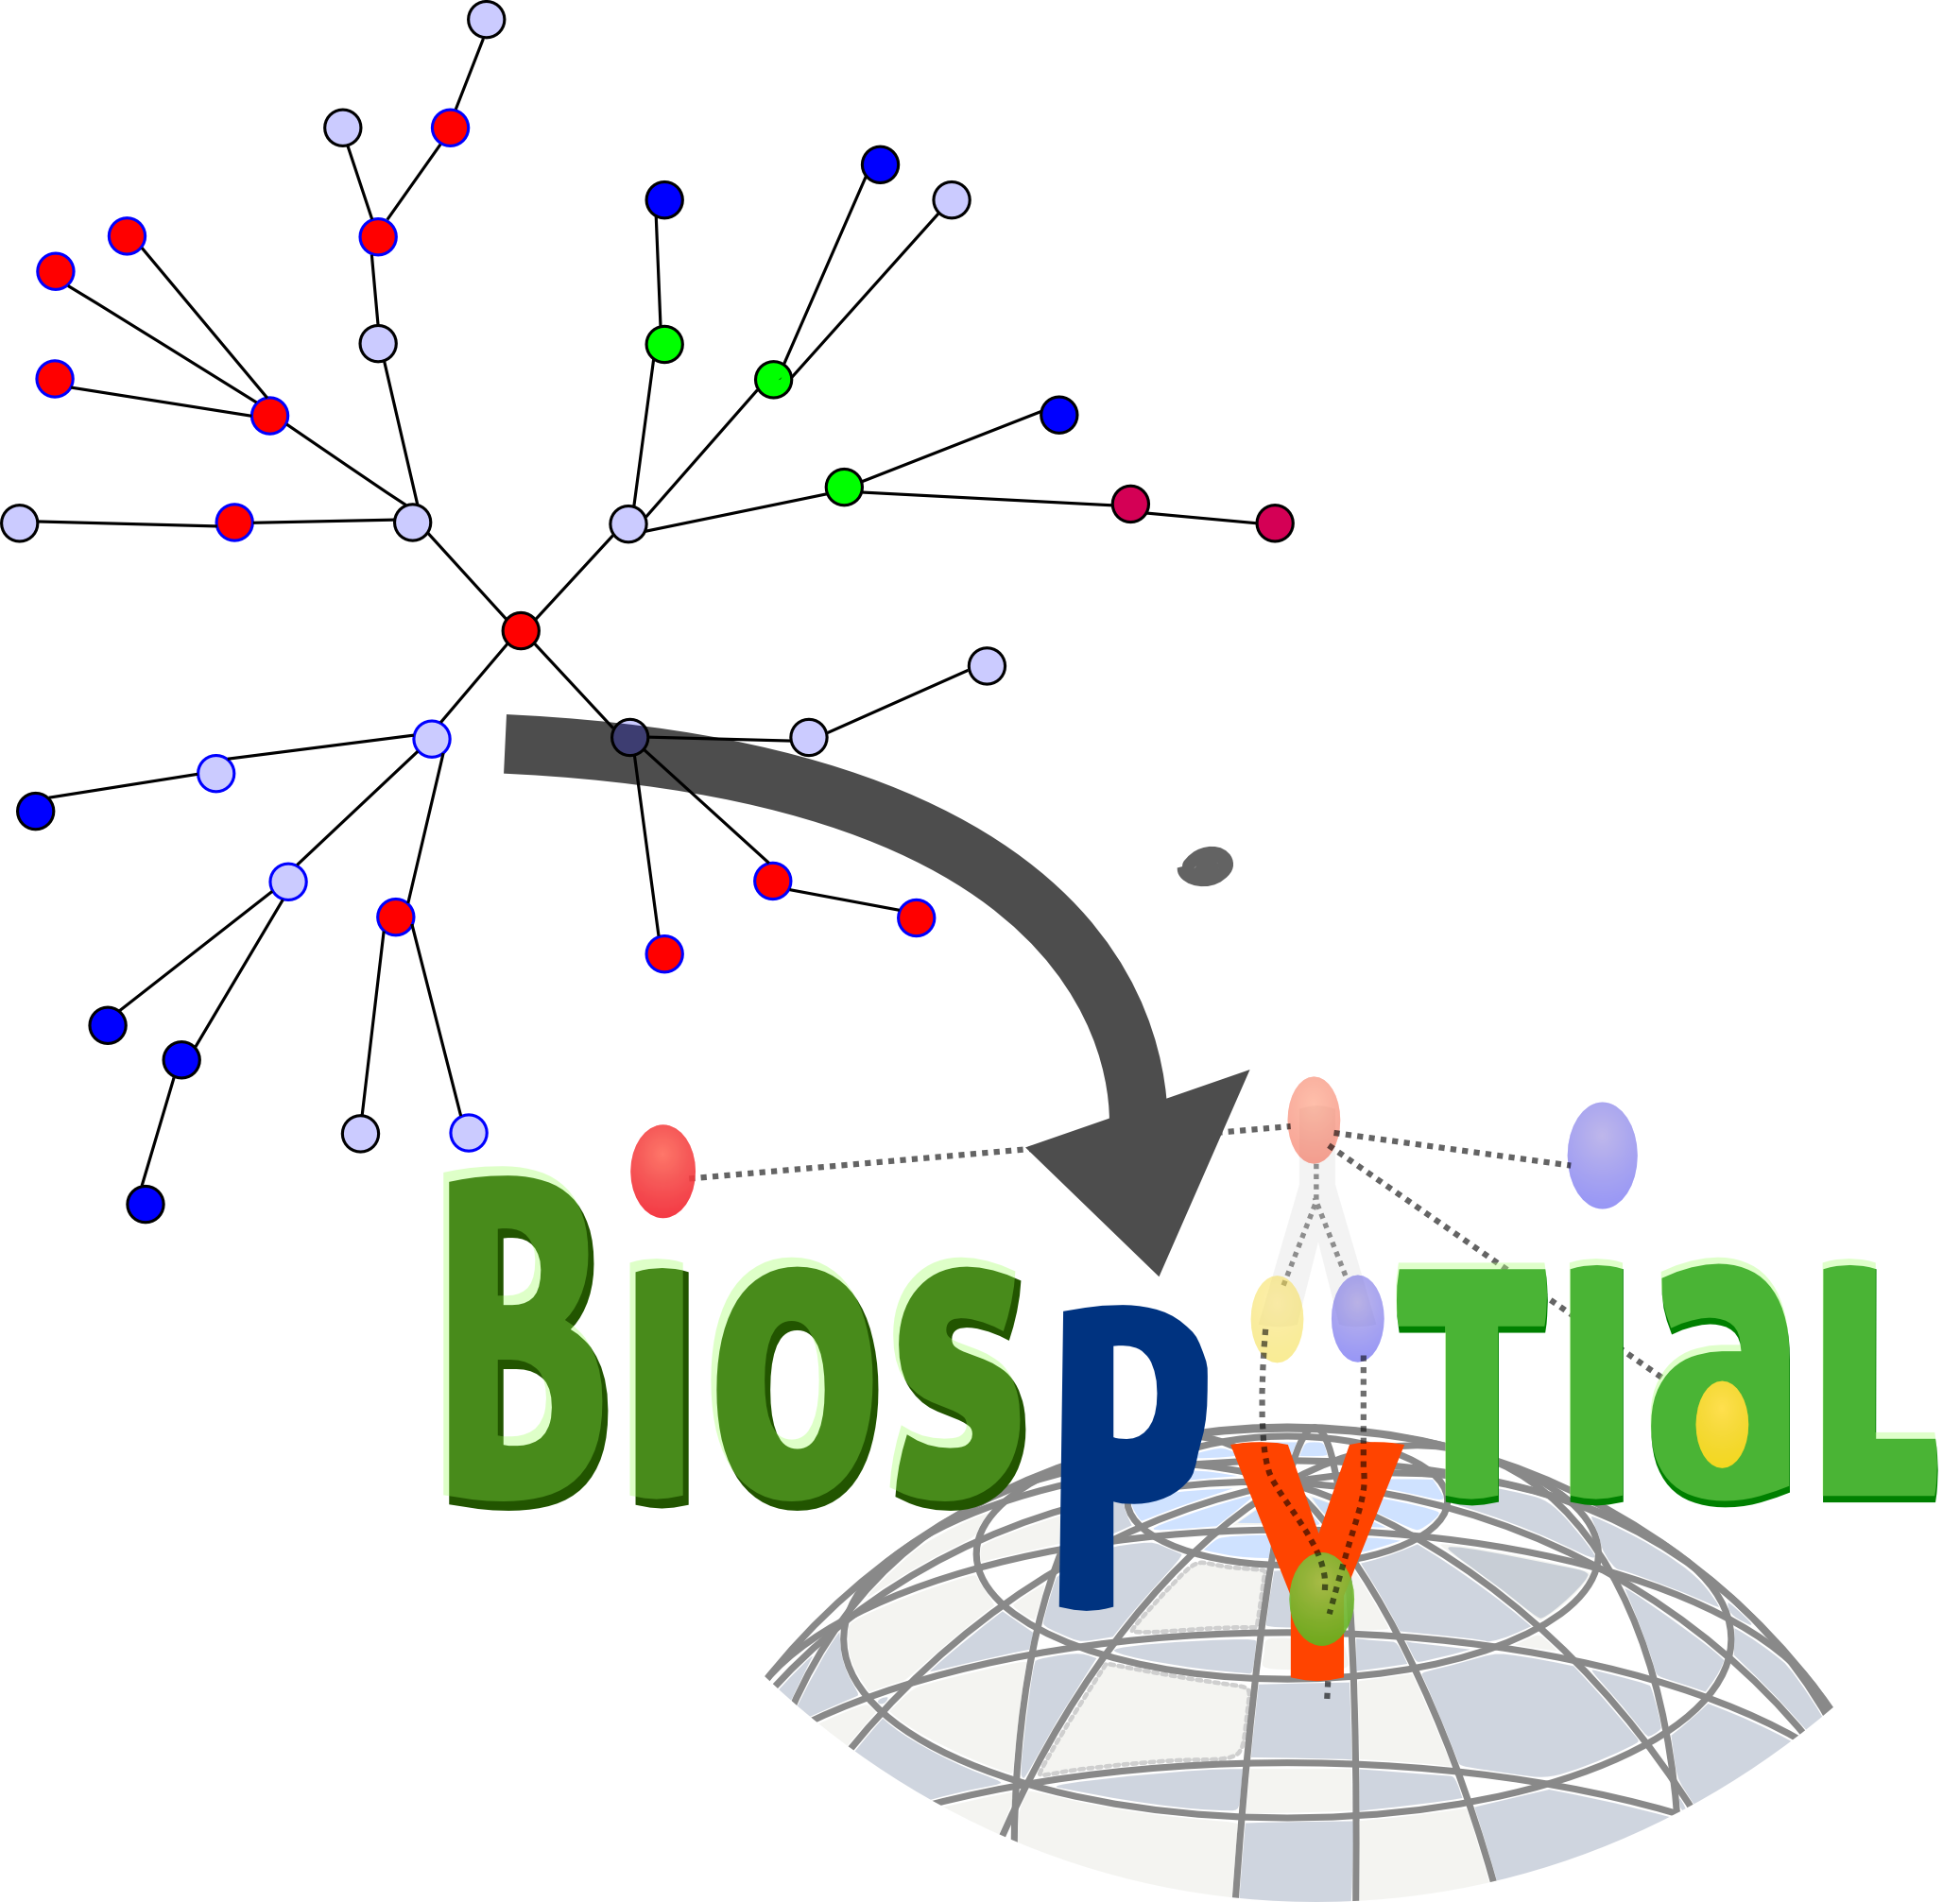
\includegraphics[scale=0.3]{graph-model3.png}}
\end{frame}

\subsection{Architecture}
\begin{frame}{What is Biospytial ?}
\begin{block}{A Graph engine}
that integrates raster and vector data in explicit relational structures. (i.e. Networks / Graphs ).\\
\centering
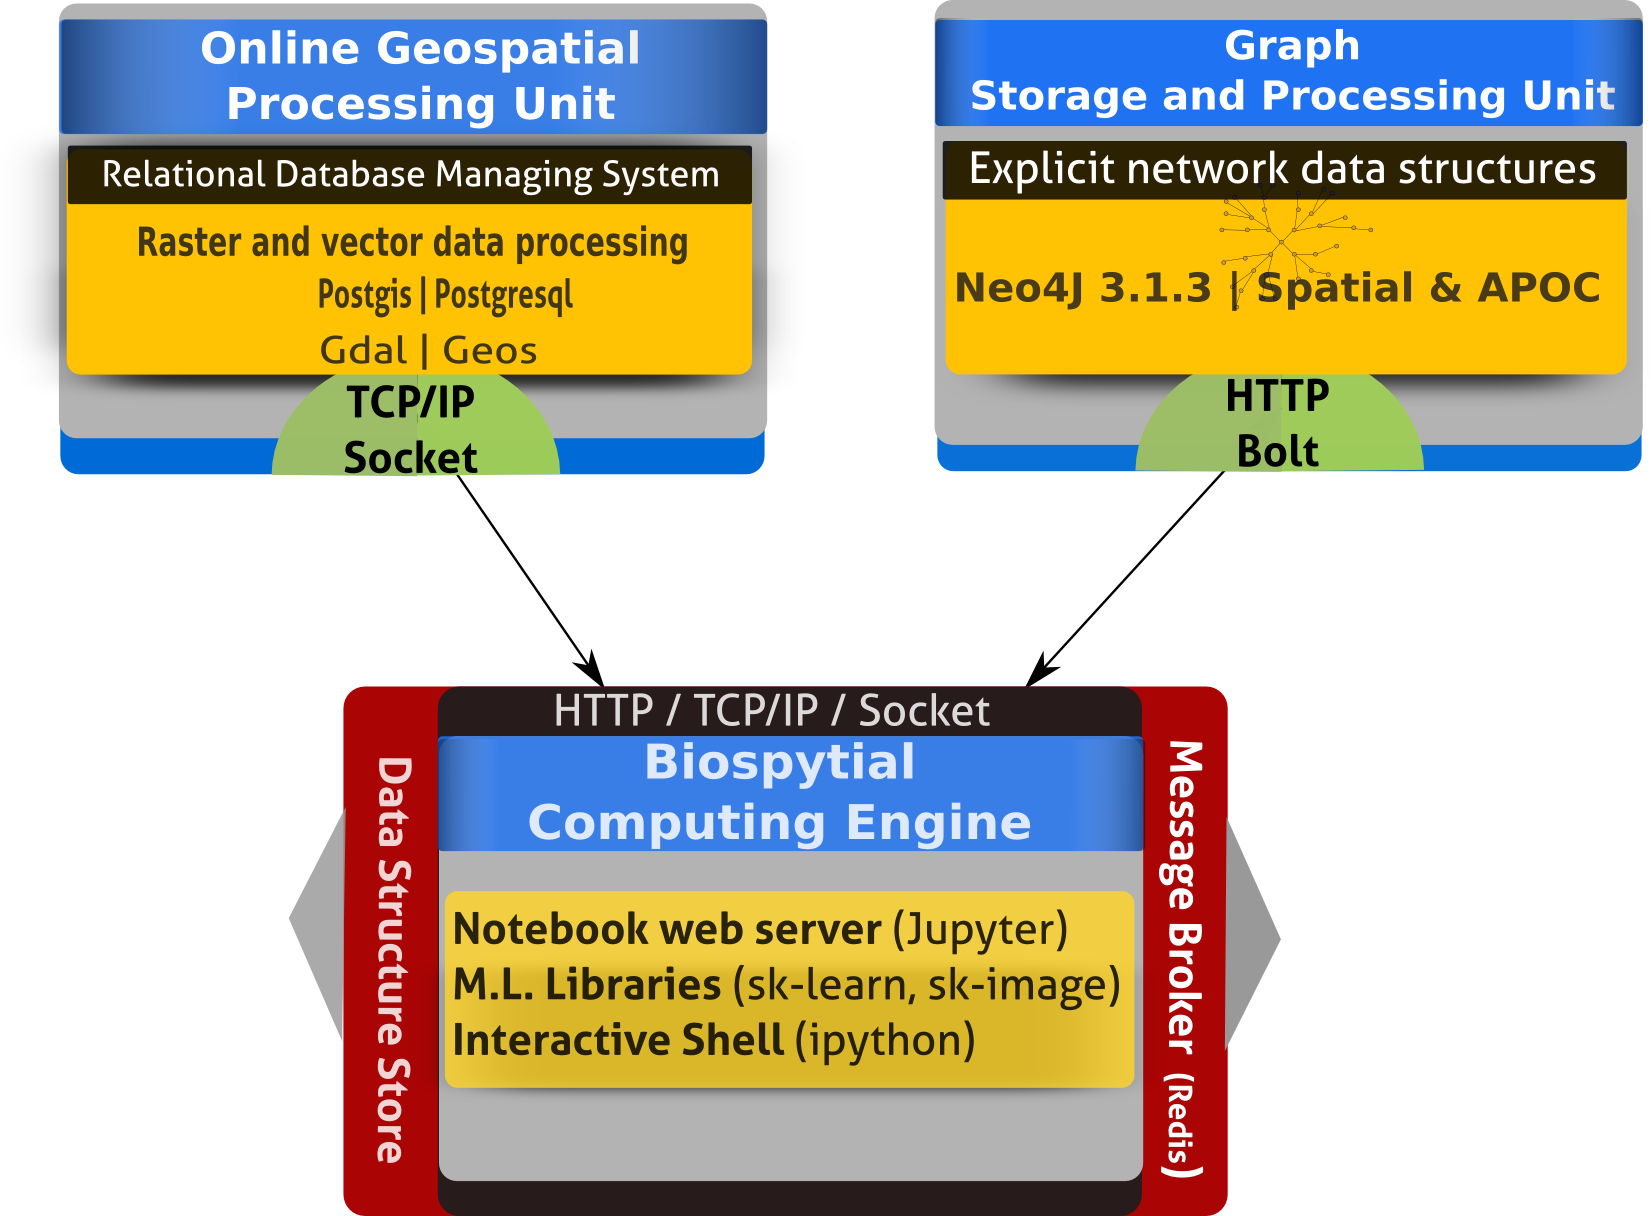
\includegraphics[scale=0.35]{biospytial-stack.png}

\end{block}
\end{frame}
\subsection{Supported Data}
\begin{frame}
\frametitle{Vector data (points,lines,(multi)-polygons}
\begin{columns}
	\begin{column}{0.3\textwidth}
	\begin{block}{Attributes}						
		\begin{itemize}
	\item id: Integer 
	\item species id : Integer
	\item level: Integer
	\item latitude / longitude: float
	\item event date: DateTime
	\item name: String
	\item pk: 2406040
	\item geom: WKT 
	\item levelname: String
\end{itemize}							
	\end{block}		
	\end{column}	
			\begin{column}{0.7\textwidth}
			\centering
	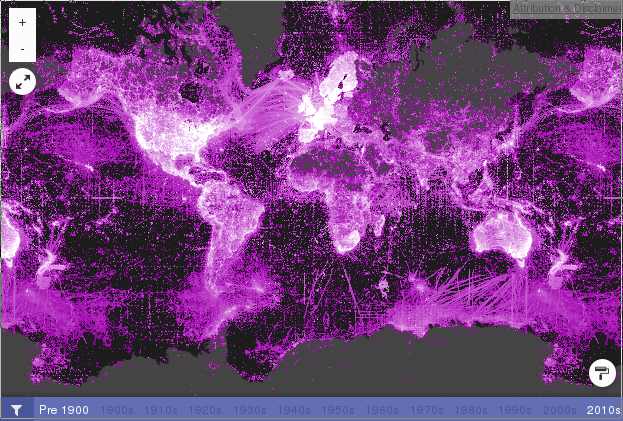
\includegraphics[scale=0.5]{gbif.png} 
	{\tiny GBIF (Global Biodiversity Information Facility) {\tt www.gbif.org} The data is a join effort in collecting all the publicly available data on biodiversity in the planet. This snapshot is from September, 2013}	
		    \end{column}    	    
		\end{columns}					
	\end{frame}	




\begin{frame}{Environmental Data}
\begin{columns}
	\begin{column}{0.4\textwidth}
\begin{block}{BioClim - Datasource}
Bioclimatic variables derived from monthly data 1978 -  2000 \\(12 Months, 30arc res.)
\begin{itemize}
	\item Temperature (Max, Mean, Min)
	\item Precipitation
	\item Wind Speed
	\item Vapor Pressure
	\item Solar Radiation
	\item DEM-based (Aspect, Slope, Height)
\end{itemize}
	\end{block}		
	\end{column}
	\begin{column}{0.6\textwidth}
			\centering
			\centering
\animategraphics[controls,scale=0.2]{2}{meantemp-}{0}{11}
{\tiny \\ Hijmans, R.J., S.E. Cameron, J.L. Parra, P.G. Jones and A. Jarvis, 2005. Very high resolution interpolated climate surfaces for global land areas. International Journal of Climatology 25: 1965-1978. * }
\end{column}    	    
		\end{columns}	
\end{frame}

\section{Algorithms}

\begin{frame}
\frametitle{The taxonomy as a partial order $\leq$ }
\begin{columns}[t]
        \column{.5\textwidth}
        \centering
        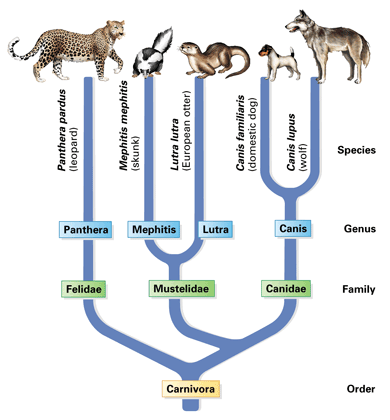
\includegraphics[width=0.6\columnwidth,height=2.5cm]{mamalia.png}
        \captionof{figure}{Common ancestor}
		\centering		
		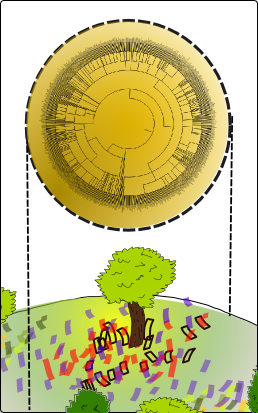
\includegraphics[width=0.6\columnwidth,height=2.5cm]{build_tree.png}
        \captionof{figure}{Tree structure}
        \column{.5\textwidth}
		\centering        
        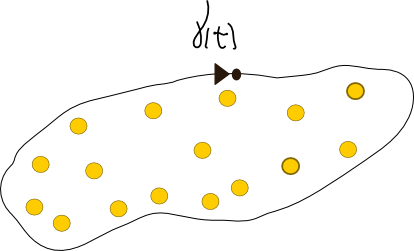
\includegraphics[width=0.6\columnwidth,height=2.5cm]{area_occs.png}
        \captionof{figure}{Occurrences contained in:...}
		\centering        
        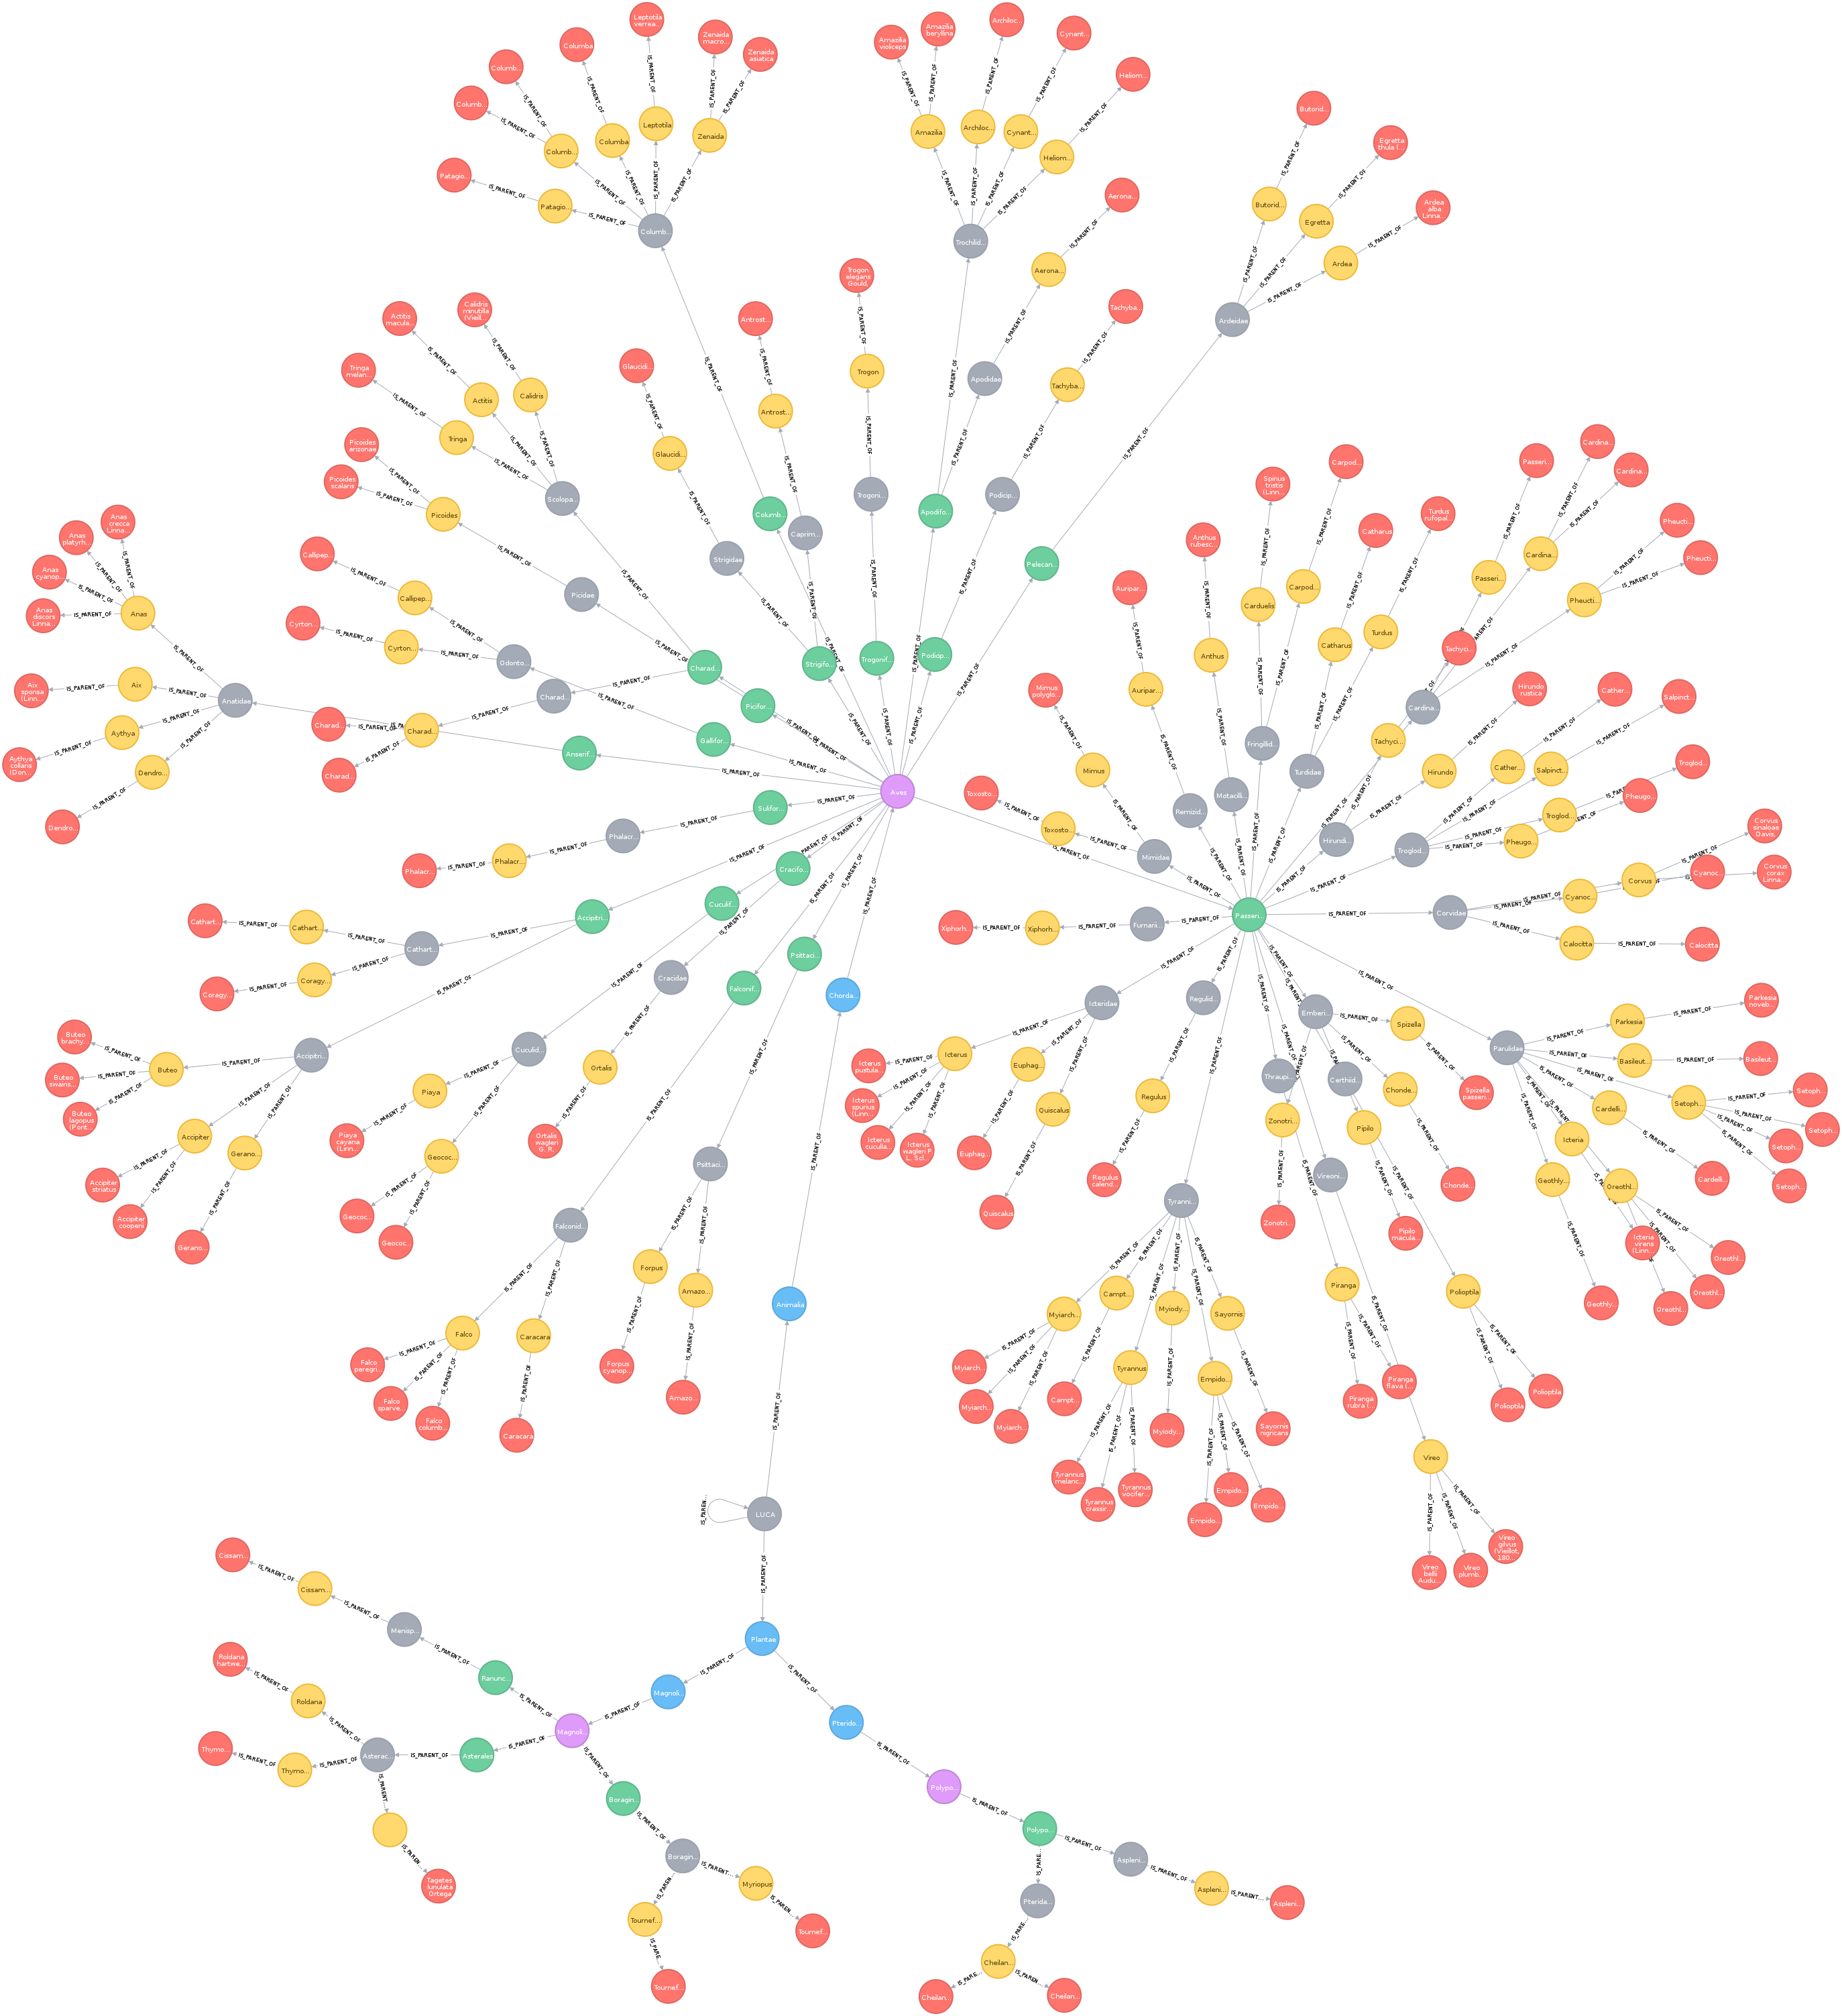
\includegraphics[width=0.6\columnwidth,height=2.5cm]{tree.png}
        \captionof{figure}{A sub-tree of the Tree of Life}
\end{columns}						
	\end{frame}	


\subsection{Nested Grids}
\subsubsection{Spatial Lattice}
\begin{frame}
\frametitle{spatial Semi-lattice }
\begin{columns}[t]
        \column{.5\textwidth}
		\centering		
		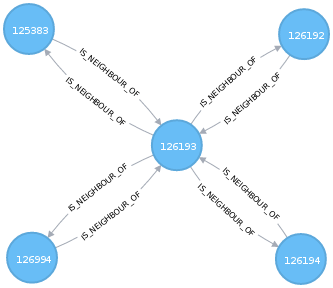
\includegraphics[width=0.6\columnwidth,height=2.5cm]{cell_neighbours.png}
        \captionof{figure}{An area cell an its neighbours}
        \centering
        
\includegraphics[width=0.6\columnwidth,height=2.5cm]{gridtest1.png}
		\captionof{figure}{A lattice}           
        \column{.5\textwidth}
		\centering        
        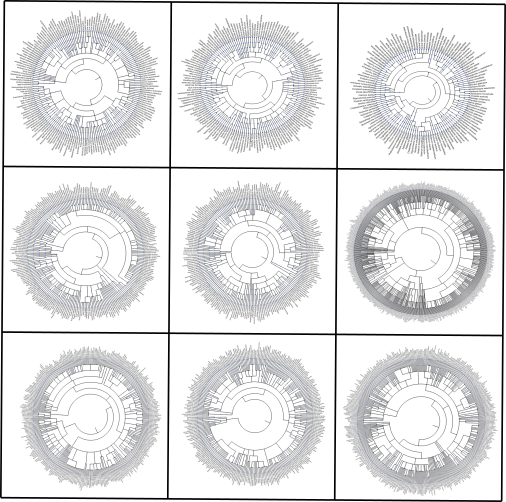
\includegraphics[width=0.6\columnwidth,height=2.5cm]{griddedtaxonomy.png}
        \captionof{figure}{{\em On every cell a tree}}
		\centering        
        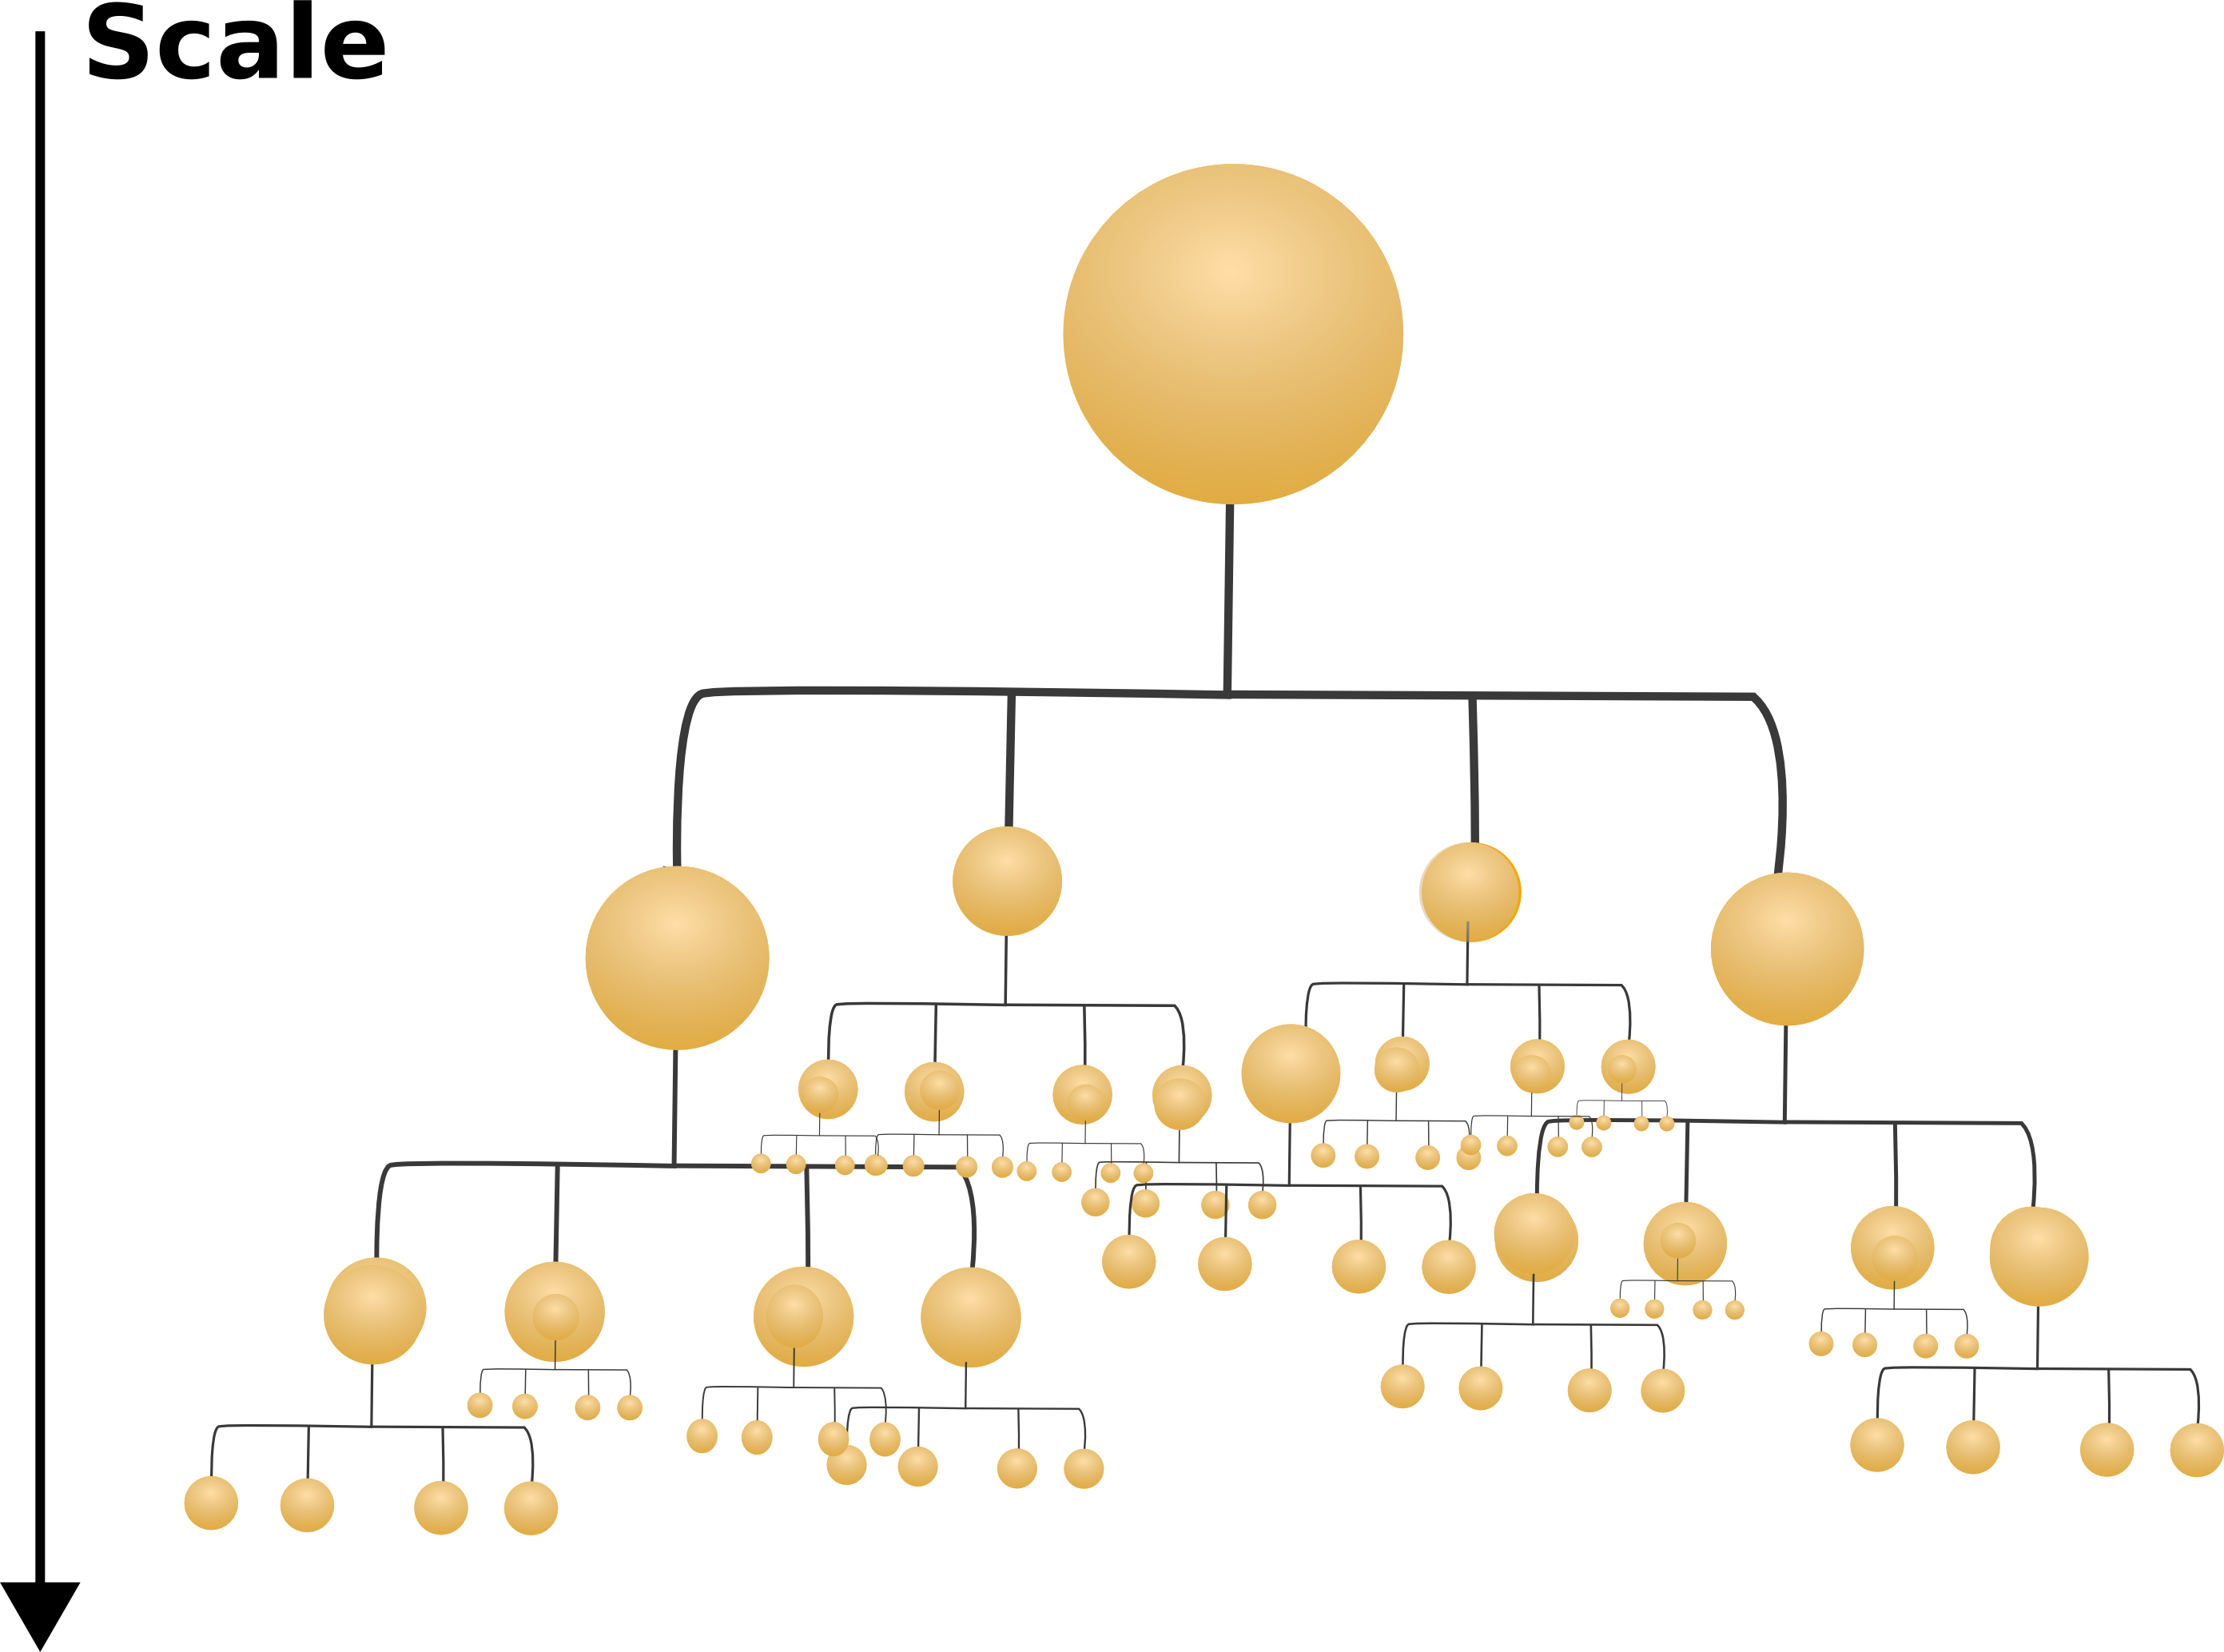
\includegraphics[width=0.6\columnwidth,height=2.5cm]{quadtree.png}
        \captionof{figure}{Another tree across scale}
\end{columns}						
	\end{frame}	





\subsection{Monoids on Trees}
\begin{frame}{Tree operations}
\begin{block}{Semigroup}
Let $T$ be a set and $m : T \times T \rightarrow T $ be an associative binary operation\footnote{Meaning that if $t,p,q \in T$ then $m(m(t,p),q) = m(t,m(p,q))$ }. 
The duple $(T,m)$ is called a semigroup and $T$ is called the underlying set of the semigroup.
\end{block}

\begin{block}{Identity element}
Let $e \in T$ and $T$ a semigroup. $e$ is called {\em identity element} if and only if $te = et$ for all $t \in T$. There can only be at most one identity element in a semigroup.
\end{block}
\end{frame}

\begin{frame}
\begin{block}{Monoid}
A {\em monoid} is a set that is {\bf closed} under the associative operation of a semigroup with an identity element.
	\end{block}
	The $+$ and $-$ operator of taxonomic trees are monoids.
		\centering
	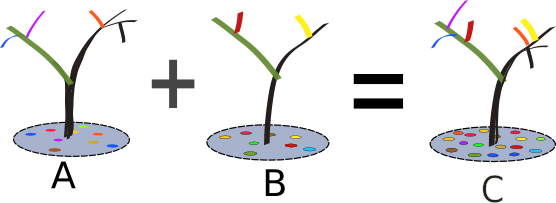
\includegraphics[scale=1]{sum_monoid.png} 
\end{frame}

\begin{frame}{Operations}
	\begin{block}{Other available operations}
	\centering
	\includegraphics<1>[scale=1.5]{operators.png} 

	\end{block}
\end{frame}
\section{Demo}
\begin{frame}{Some Demo}
\begin{block}

\end{block}
\end{frame}
\section{Code and contaners}

\begin{frame}{Code and container availability}

\end{frame}
\end{document}
